\documentclass[tikz,border=8pt]{standalone}
% Shared look for every TikZ diagram. Load with % Shared look for every TikZ diagram. Load with % Shared look for every TikZ diagram. Load with \input{../../tools/tikz-style.tex}
\usepackage[T1]{fontenc}
\usepackage{lmodern}
\renewcommand{\sfdefault}{lmr}  % diagrams use the same serif as the text
\usetikzlibrary{arrows.meta, positioning, shapes.geometric, calc, fit, backgrounds}
\definecolor{cblue}{HTML}{4C78A8}
\definecolor{corange}{HTML}{F58518}
\definecolor{cgreen}{HTML}{54A24B}
\definecolor{cred}{HTML}{E45756}
\definecolor{cpurple}{HTML}{B279A2}
\definecolor{cgrey}{HTML}{6B6B6B}
\tikzset{
  every picture/.style={font=\sffamily, line width=1.2pt},
  box/.style={draw=#1, fill=#1!12, rounded corners=4pt, align=center, inner sep=7pt, minimum height=1.1cm},
  box/.default=cgrey,
  arrow/.style={-{Stealth[length=3mm]}, draw=cgrey, line width=1.4pt},
  title/.style={font=\sffamily\bfseries\Large},
  note/.style={font=\sffamily\small, text=cgrey, align=center},
}
\AtBeginDocument{\hyphenpenalty=10000 \exhyphenpenalty=10000}

\usepackage[T1]{fontenc}
\usepackage{lmodern}
\renewcommand{\sfdefault}{lmr}  % diagrams use the same serif as the text
\usetikzlibrary{arrows.meta, positioning, shapes.geometric, calc, fit, backgrounds}
\definecolor{cblue}{HTML}{4C78A8}
\definecolor{corange}{HTML}{F58518}
\definecolor{cgreen}{HTML}{54A24B}
\definecolor{cred}{HTML}{E45756}
\definecolor{cpurple}{HTML}{B279A2}
\definecolor{cgrey}{HTML}{6B6B6B}
\tikzset{
  every picture/.style={font=\sffamily, line width=1.2pt},
  box/.style={draw=#1, fill=#1!12, rounded corners=4pt, align=center, inner sep=7pt, minimum height=1.1cm},
  box/.default=cgrey,
  arrow/.style={-{Stealth[length=3mm]}, draw=cgrey, line width=1.4pt},
  title/.style={font=\sffamily\bfseries\Large},
  note/.style={font=\sffamily\small, text=cgrey, align=center},
}
\AtBeginDocument{\hyphenpenalty=10000 \exhyphenpenalty=10000}

\usepackage[T1]{fontenc}
\usepackage{lmodern}
\renewcommand{\sfdefault}{lmr}  % diagrams use the same serif as the text
\usetikzlibrary{arrows.meta, positioning, shapes.geometric, calc, fit, backgrounds}
\definecolor{cblue}{HTML}{4C78A8}
\definecolor{corange}{HTML}{F58518}
\definecolor{cgreen}{HTML}{54A24B}
\definecolor{cred}{HTML}{E45756}
\definecolor{cpurple}{HTML}{B279A2}
\definecolor{cgrey}{HTML}{6B6B6B}
\tikzset{
  every picture/.style={font=\sffamily, line width=1.2pt},
  box/.style={draw=#1, fill=#1!12, rounded corners=4pt, align=center, inner sep=7pt, minimum height=1.1cm},
  box/.default=cgrey,
  arrow/.style={-{Stealth[length=3mm]}, draw=cgrey, line width=1.4pt},
  title/.style={font=\sffamily\bfseries\Large},
  note/.style={font=\sffamily\small, text=cgrey, align=center},
}
\AtBeginDocument{\hyphenpenalty=10000 \exhyphenpenalty=10000}

\usetikzlibrary{matrix}
% Section 4.2: z1 = W1^T a0 + b1. Row j of W1^T (= column j of W1) meets a0 and gives the sum for node j.
% Row products: 0.330, -0.330, 0.447; plus bias 0.1, -0.1, 0.2 -> 0.430, -0.430, 0.647.
\begin{document}
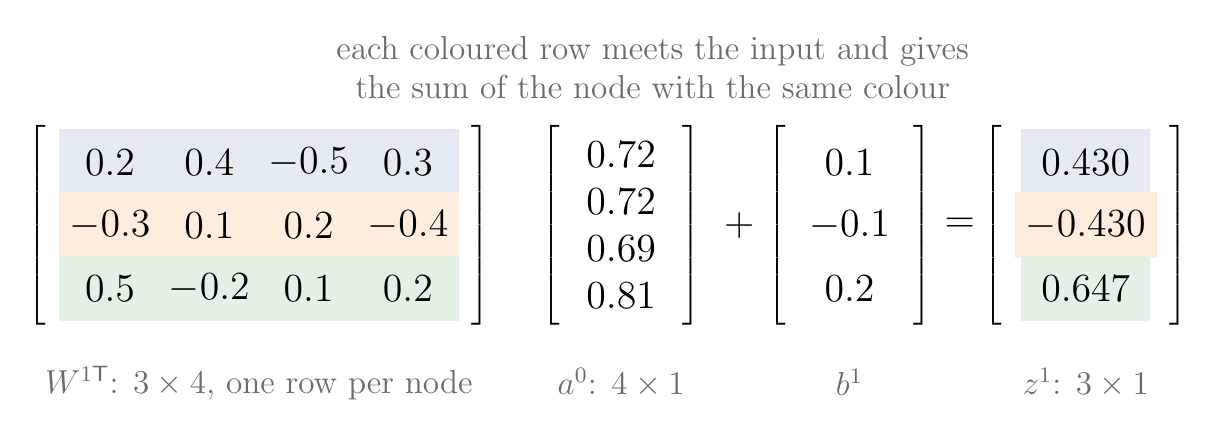
\begin{tikzpicture}[every node/.append style={font=\Large}]
  \matrix (W) [matrix of math nodes, nodes={minimum width=1.25cm, minimum height=0.8cm, anchor=center}, left delimiter={[}, right delimiter={]}] at (0,0) {
    0.2 & 0.4 & -0.5 & 0.3 \\ -0.3 & 0.1 & 0.2 & -0.4 \\ 0.5 & -0.2 & 0.1 & 0.2 \\ };
  \begin{scope}[on background layer]
    \fill[cblue!15] (W-1-1.north west) rectangle (W-1-4.south east);
    \fill[corange!15] (W-2-1.north west) rectangle (W-2-4.south east);
    \fill[cgreen!15] (W-3-1.north west) rectangle (W-3-4.south east);
  \end{scope}
  \matrix (a) [matrix of math nodes, nodes={minimum width=1.2cm, minimum height=0.6cm}, left delimiter={[}, right delimiter={]}] at (4.6,0) {
    0.72 \\ 0.72 \\ 0.69 \\ 0.81 \\ };
  \node at (6.1, 0) {$+$};
  \matrix (b) [matrix of math nodes, nodes={minimum width=1.2cm, minimum height=0.8cm}, left delimiter={[}, right delimiter={]}] at (7.5,0) {
    0.1 \\ -0.1 \\ 0.2 \\ };
  \node at (8.9, 0) {$=$};
  \matrix (z) [matrix of math nodes, nodes={minimum width=1.6cm, minimum height=0.8cm}, left delimiter={[}, right delimiter={]}] at (10.5,0) {
    0.430 \\ -0.430 \\ 0.647 \\ };
  \begin{scope}[on background layer]
    \fill[cblue!15] (z-1-1.north west) rectangle (z-1-1.south east);
    \fill[corange!15] (z-2-1.north west) rectangle (z-2-1.south east);
    \fill[cgreen!15] (z-3-1.north west) rectangle (z-3-1.south east);
  \end{scope}
  \node[note, font=\large] at (0, -2.0) {$W^{1\mathsf T}$: $3 \times 4$, one row per node};
  \node[note, font=\large] at (4.6, -2.0) {$a^{0}$: $4 \times 1$};
  \node[note, font=\large] at (7.5, -2.0) {$b^{1}$};
  \node[note, font=\large] at (10.5, -2.0) {$z^{1}$: $3 \times 1$};
  \node[note, font=\large, text width=13cm] at (5, 2.0) {each coloured row meets the input and gives the sum of the node with the same colour};
\end{tikzpicture}
\end{document}
